\chapter{Evaluación}
\label{cap:evaluacion}



\begin{resumen}
	 En este capítulo se explicará el proceso de evaluación de la aplicación: Empezando por la preparación (Sección \ref{eva:prep}), el diseño de la evaluación (Sección \ref{eva:dis}), resultados obtenidos (Sección \ref{eva:res}) y el análisis de dichos resultados (Sección \ref{eva:analisis}).  
	
\end{resumen}

Al tener un prototipo funcional con la suficiente antelación a la entrega, se puso en marcha el plan de realizar una evaluación con usuarios. Durante este mes se focalizó el trabajo en mejorar la usabilidad e interfaz de la aplicación, diseñar la evaluación y en dar a conocer la aplicación al público objetivo de la aplicación. Éstos son usuarios creadores de material pictográfico, generalmente profesores de educación especial y padres y tutores. 


\section{Preparación de la evaluación}
\label{eva:prep}


Inicialmente se buscaron sitios donde se subiera material pictográfico con frecuencia para así localizar a los creadores de dicho material y contactar con ellos. La propia web de ARASAAC cuenta con una sección dedicada a la subida de material pictográfico donde se añaden nuevo material diariamente. La la inmensa mayoría de este material contaba con una marca de agua indicando el perfil de Instagram del creador. Por ello nos decantamos por \textbf{crear una cuenta de Instagram\footnote{\url{https://www.instagram.com/pictupweb/}} para crear una red de potenciales usuarios}. 

En dicha cuenta, se contactó con muchos de estos creadores de material para informarles sobre el desarrollo de la aplicación. También se creó \textbf{material en forma de vídeos} donde se explicaban muchas funcionalidades de la web. Los vídeos contaron con una recepción positiva y de interés por parte de los usuarios, por lo que en el transcurso del mes se logró un grupo considerable de usuarios.
\section{Diseño de la evaluación}
\label{eva:dis}

Es en este punto donde la situación causada por la situación de pandemia tuvo mayor impacto sobre el proyecto. En otras circunstancias la evaluación hubiera sido en un centro escolar de manera más cercana al usuario final, es por ello que se tuvo que plantear una \textbf{evaluación a distancia y asíncrona}. \textbf{El objetivo de esta evaluación es medir la usabilidad y utilidad de la aplicación}. 


Debido a estas circunstancias, la evaluación se realizó mediante un formulario para que el usuario pudiera completarlo por su cuenta. Por contraposición también estaba la posibilidad que el usuario dejara el formulario incompleto en caso de no lograr completar alguna tarea. Otro problema es el dispositivo de evaluación, ya que la aplicación está diseñada y probada para ordenadores. Por ello antes y durante la realización del formulario se aconsejó encarecidamente el uso del ordenador para el desarrollo de la evaluación. 

Primero se plantean algunas\textbf{ preguntas para conocer la relación de los usuarios respecto al uso de pictogramas}, la edad y ocupación. De esta manera se podría determinar el tipo de perfil de usuario que está evaluando.

Tras conocer el perfil, se plantean una serie de\textbf{ tareas a realizar} dentro de la aplicación. Antes de plantear las tareas, se vuelve a recomendar al usuario el uso de ordenador para probar la web. Respecto al  posible escenario en el cual el usuario no supiera continuar con la tarea y dejara el formulario incompleto, fue solucionado mediante \textbf{pistas}. Las pistas son imágenes autoexplicativas donde se especifican las acciones que se han de realizar para completar cada tarea. Como se puede ver en la Figura \ref{fig:evaPista}, se trata de la pista que indica cómo buscar un pictograma.

\begin{figure}[h!]
	\centering
	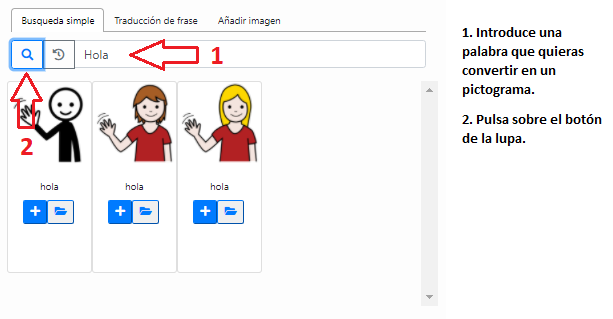
\includegraphics[width=0.8\linewidth]{Imagenes/Bitmap/evaluacionPista}
	\caption{ Ejemplo de pista en el formulario: Buscar un pictograma.
	}
	\label{fig:evaPista}
\end{figure} 

En el formulario las pistas vienen dadas mediante una pregunta que se podría realizar el usuario de cara a completar una tarea, seguido de una URL que redirige a la imagen de la pista asociada. De esta manera el usuario puede resolver una duda concreta y \textbf{no se desvela cómo completar otras acciones dentro de la tarea}. Otra manera de orientar al usuario a saber si ha realizado una tarea correctamente fue mediante imágenes que mostraran un posible estado final del tablero o componente al completar la tarea. 


Respecto a las tareas, aunque no se abarcan todas las posibilidades, representa una muestra significativa de las funcionalidades disponibles en la aplicación. Esto se debe a que el formulario debe de completarse en un período razonable de tiempo y no extenderse más de lo debido. 
A continuación se detallarán las tareas escogidas y el motivo de elección: 

\begin{itemize}
	\item \textbf{Buscar un pictograma, añadirlo al tablero y editarlo}: Se trata de la funcionalidad más básica de la aplicación.
	\item \textbf{Crear una lista de pictos, añadir un pictograma a una lista de pictos y añadir un pictograma de la lista al tablero}: Una funcionalidad que ha causado dudas durante el desarrollo ya que se desconocía si era lo suficientemente claro su funcionamiento.
	\item \textbf{Traducir una frase, añadirla al tablero y ocultar un pictograma de la frase}: Al ser una funcionalidad más compleja y más opciones era deseable conocer el desempeño del usuario con ésta.
	\item \textbf{Añadir fotos, figuras e iconos al tablero}: Abarcan funciones independientes más simples comparadas con las anteriores, ya que requieren menos acciones para completarlas.
\end{itemize}
El tipo de cuestionario seleccionado para medir la usabilidad de cada tarea ha sido el \textbf{ASQ\footnote{\url{https://help.qualaroo.com/hc/en-us/articles/360039070552-After-Scenario-Questionnaire-ASQ-}}} (After Scenario Cuestionare), el cual permite al usuario evaluar la dificultad de cada una. Este cuestionario ha de ser respondido una vez finalizada cada tarea y está compuesta por tres afirmaciones. El usuario ha de indicar cuán de acuerdo está mediante una escala de 1 a 7, siendo el 1 muy en desacuerdo y el 7 muy de acuerdo. Dichas afirmaciones son: 

\begin{enumerate}
	\item En general, estoy satisfecho con la facilidad para completar la tarea en este escenario.
	\item En general, estoy satisfecho con la cantidad de tiempo que tomó completar la tarea en este escenario.
	\item Estoy satisfecho con la respuesta de la web al realizar una acción, sé lo que pasa en todo momento
\end{enumerate}

Esta última afirmación fue modificada para ser ajustada al contexto de la aplicación, enfocándose más al feedback que pueda aportar la tarea. Originalmente ésta era:  \textit{En general, estoy satisfecho con la información de soporte (ayuda en línea, mensajes y documentación) al completar la tarea}

Tras completar las tareas, se ofrece al usuario a que siga probando la aplicación con libertad para probar el resto de funcionalidades que no aparecieran en las tareas.  
También se dejan un hueco de respuesta libre en función si se ha sentido perdido o ha echado en falta alguna función durante la realización de las tareas. 

Por último, de manera opcional se propone al usuario otro formulario donde puede dar su opinión sobre la aplicación de manera global. Para ello se ha utilizado las preguntas de la escala SUS\footnote{\url{https://help.qualaroo.com/hc/en-us/articles/360039474571-System-Usability-Scale-SUS-}} (System Usability Scale), que mide la usabilidad del sistema. Nuevamente plantea una serie de afirmaciones, en este caso 10 donde el usuario deberá elegir en una escala de 1 a 5 cuán de acuerdo está con ellas. Dichas afirmaciones son: 


\begin{enumerate}
	\item Creo que usaría esta web frecuentemente
	\item Encontré la web innecesariamente compleja
	\item Creo que la web es fácil de usar
	\item Creo que necesitaría la ayuda de una persona con conocimientos técnicos para usar la web
	\item Las funciones de la web están bien integradas
	\item Creo que la web es muy confusa
	\item Creo que la mayoría de la gente aprendería a usar la web muy rápidamente
	\item Encuentro la web muy complicada de utilizar
	\item Me siento confiado/a al utilizar la web
	\item Necesito aprender muchas cosas antes de poder utilizar la web
\end{enumerate}

Una vez acabado el cuestionario, éste fue enviado, tras dos semanas, se obtuvieron más de 35 respuestas por parte de estudiantes y profesores. 

Continuará...

\section{Resultados de la evaluación}
\label{eva:res}

\section{Análisis de los resultados}
\label{eva:analisis}


\begin{tabular}{ |p{4cm}|p{2cm}|p{2cm}|p{2cm}|p{2cm}|  }
	\hline
	\multicolumn{5}{|c|}{Tarea 1} \\
	\hline
	 & \multicolumn{2}{|p{4cm}|}{Grupo de usuarios que crean y usan material pictográfico} & \multicolumn{2}{|p{4cm}|}{Grupo del resto de usuarios }  \\ 
	\hline
	 Preguntas ASQ & Puntuación media  &Desviación típica de la puntuación & Puntuación media & Desviación típica de la puntuación\\
	\hline
	1. En general, estoy satisfecho con la facilidad de completar esta tarea &  & &  &\\
	\hline
	2. En general estoy satisfecho con la cantidad de tiempo que me ha llevado completar esta tarea&  &  & &\\
	\hline
	3. Estoy satisfecho con la respuesta de la web al realizar una acción, sé lo que pasa en todo momento & & &   &\\
	\hline
	Nota final & & &  &\\
	\hline
	\multicolumn{5}{|c|}{Uso de pistas en Tarea 1} \\
	\hline
	& \multicolumn{2}{|p{4cm}|}{Grupo de usuarios que crean y usan material pictográfico} & \multicolumn{2}{|p{4cm}|}{Grupo del resto de usuarios }  \\ 
	\hline
	 Pistas &Nº de usos de la pista &\% de uso de la pista&Nº de usos de la pista&\% de uso de la pista\\
	\hline
	Pista 1: Buscar pictograma &  & &  &\\
	\hline
	Pista 2: Añadir al tablero &  &  & &\\
	\hline
	Pista 3: Editar picto & & &   &\\
	\hline
\end{tabular}
